\begin{figure}[H]
    \centering
    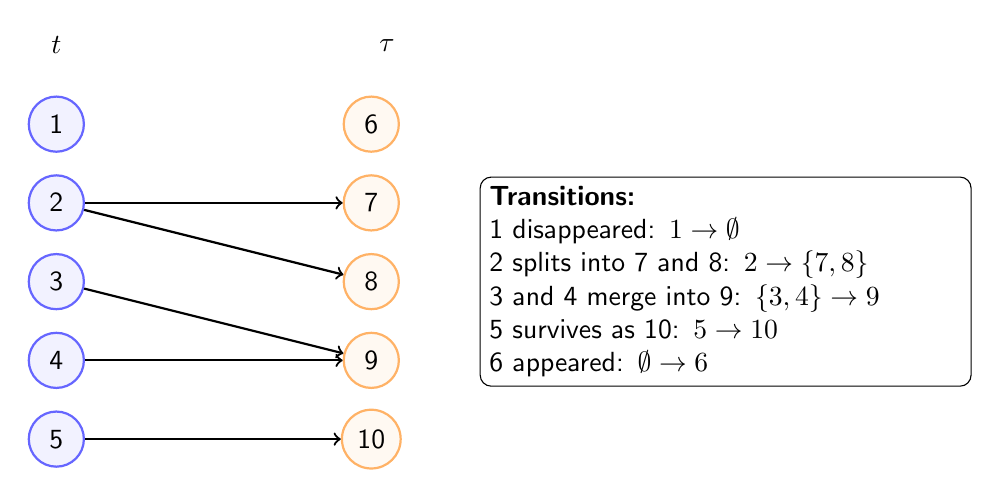
\begin{tikzpicture}[
            leftnode/.style={circle, draw=blue!60, fill=blue!5, thick, minimum size=7mm},
            rightnode/.style={circle, draw=orange!60, fill=orange!5, thick, minimum size=7mm},
            font=\sffamily,
            node distance=8mm and 30mm
        ]

        % Time labels
        \node[font=\bfseries] at (0,2) {$t$};
        \node[font=\bfseries] at (4.2,2) {$\tau$};

        % Left nodes (1 to 5)
        \node[leftnode] (n1) at (0,1) {1};
        \node[leftnode] (n2) at (0,0) {2};
        \node[leftnode] (n3) at (0,-1) {3};
        \node[leftnode] (n4) at (0,-2) {4};
        \node[leftnode] (n5) at (0,-3) {5};

        % Right nodes (6 to 10)
        \node[rightnode] (n6) at (4,1) {6};
        \node[rightnode] (n7) at (4,0) {7};
        \node[rightnode] (n8) at (4,-1) {8};
        \node[rightnode] (n9) at (4,-2) {9};
        \node[rightnode] (n10) at (4,-3) {10};

        % Edges
        \draw[->, thick] (n2) -- (n7);
        \draw[->, thick] (n2) -- (n8);
        \draw[->, thick] (n3) -- (n9);
        \draw[->, thick] (n4) -- (n9);
        \draw[->, thick] (n5) -- (n10);

        % Transitions legend centered vertically
        \node[align=left, anchor=center, text width=6cm, draw, rounded corners] (legend) at (8.5,-1) {
            \textbf{Transitions:} \\
            1 disappeared: $1 \rightarrow \emptyset$ \\
            2 splits into 7 and 8: $2 \rightarrow \{7, 8\}$ \\
            3 and 4 merge into 9: $\{3, 4\} \rightarrow 9$ \\
            5 survives as 10: $5 \rightarrow 10$ \\
            6 appeared: $\emptyset \rightarrow 6$
        };

    \end{tikzpicture}
    \caption{Example of transitions from clusters at time $t$ to clusters at time $\tau$.}
    \label{fig:cluster-transitions}
\end{figure}